\documentclass[a4paper, 11pt]{scrartcl}
 \usepackage[ngerman]{babel}
 \usepackage{graphicx}
 \usepackage{fullpage}
 \usepackage[utf8]{inputenc}
 \usepackage{amsmath}
 \usepackage{epstopdf}
 \usepackage{listings}
 \usepackage{dsfont}
 \usepackage{float}
 \usepackage{url}
 \usepackage{hyperref}
 \usepackage{subcaption}
 \usepackage{listings}
 
% To keep the font consistent across the text and the heading
 \setkomafont{sectioning}{\rmfamily\bfseries}

\graphicspath{{../plots/}}

\author{Erik Teichmann\\
Matrikelnummer 761571}
\title{Computational Physics - Schrödinger Gleichung} 


\begin{document}

%========
% Title =
%========

\let\endtitlepage\relax
\begin{titlepage}
\begin{minipage}{0.5\textwidth}
\begin{flushleft}
\makeatletter
Abgabedatum: \@date
\makeatother
\end{flushleft}
\end{minipage}%
%
\begin{minipage}{0.5\textwidth}
\begin{flushright}
\makeatletter
\@author\\
\makeatother
\end{flushright}
\end{minipage}

\begin{center}
\makeatletter
\Large \textbf{\underline{\@title}}
\end{center}
\makeatother
\end{titlepage}

%=============
% Einleitung =
%=============
\section{Einleitung}
Das Ziel dieses Versuches ist es, die Schrödinger-Gleichung in einem Doppelmulden-Potential zu simulieren. Dazu müssen die Eigenwerte der stationären Gleichung numerisch gefunden werden. Anschließend kann die zeitliche Entwicklung der Gleichung untersucht werden und die Richtigkeit anhand der Stationarität der Eigenfunktionen verifiziert werden.

%===========
% Methodik =
%===========
\section{Methodik}
Die zeitabhängige, dimensionslose Schrödinger-Gleichung ist durch die folgende Gleichung gegeben.
%
\begin{equation}
\hat{H} \Psi(x, t) = i \frac{\partial \Psi(x, t)}{\partial t} = \left( - \frac{\partial^2}{\partial x^2}  + V(x, t) \right) \Psi(x, t) \label{eq:time_schroed}
\end{equation}
%
Dabei ist $V(x, t)$ das Potential und $\Psi(x, t)$ die Wellenfunktion. Das verwendete Doppelmulden-Potential hat die Form ${V(x, t) = A/2(1-x^2)^2}$. Anhand der Gleichung erkennt man schnell, dass es genau zwei Nulstellen bei $\pm 1$ gibt. Diese sind unabhängig von dem Skalenparameter $A$. Im folgenden wurde $A = 1$ gewählt. Der Parameter bestimmt, wie stark das Potential ansteigt.
%
\subsection{Eigenwerte und Eigenfunktionen der stationären Schrödingergleichung} \label{sec:stat}
Zuerst wird die stationäre Schrödinger-Gleichung numerisch gelöst. Sie hat die Form
%
\begin{equation}
E \Psi(x) = \left( - \frac{\partial^2}{\partial x^2}  + V(x) \right) \Psi(x)
\end{equation}
%
$E$ ist der Eigenwert des Hamilton-Operators $\hat{H}$ und $\Psi(x)$ die zugehörige Eigenfunktion. Die Schwierigkeit bei der Lösung liegt darin, dass die Gleichung durch die Randbedingungen $\Psi(\pm \infty) = 0$ bestimmt wird.\\
Die Randbedingungen können durch geeigente Annahmen in zwei Anfangsbedingungen zerlegt werden: durch das hohe Potential kann für große $\vert x \vert$ ein Verhalten von $\Psi \propto e^{- \sqrt{E} \vert x \vert}$ angenommen werden. Es gibt also zwei Funktionen, eine linke $\Psi_{-}$ und eine  recht  $\Psi_{+}$. Das heißt die Lösungen sollten für ein großes $x_0$ die folgende Form haben:
%
\begin{align}
\Psi_{-}(x_0) & = C e^{ \sqrt{E} x_0} \\
\Psi_{+}(x_0) & = C e^{- \sqrt{E} x_0} \\
\intertext{Mit zwei Stetigkeitsbedingung}
\Psi_{+}(0) & = \Psi_{-}(0) \\
\Psi'_{+}(0) & = \Psi'_{-}(0)
\end{align}
%
Um die Differentialgleichung numerisch zu lösen werden zwei Differentialgleichungen, eine von links zu $0$ kommende mit $\Psi_{-}$ und eine von rechts zu $0$ kommende mit $\Psi_{+}$ gesucht, die die Stetigkeitsbedingung erfüllen. Um die Suche nach den Eigenwerten zu vereinfachen kann die Funktion
%
\begin{equation}
w(E) = \Psi_{+}(0)\Psi'_{-}(0) - \Psi_{-}(0)\Psi'_{+}(0) \stackrel{!}{=} 0
\end{equation}
%
verwendet werden. Die Nullstellen dieser Funktion entsprechen den Eigenwerten. Es muss darauf geachtet werden, dass die Wahl der Anfangsbedingungen immer zu einer symmetrischen Lösung führt, um antisymmetrische Lösung zu erhalten muss für die entsprechnden Eigenwerte eine der beiden Hälften mit $-1$ multipliziert werden.\\
Zur Lösung der Differentialgleichungen für $\Psi_{+}$ und $\Psi_{-}$ können typische Verfahren verwendet werden. Hier wurde ein Runge-Kutta-Verfahren der Ordnung 4 verwendet. Zur Bestimmung der Nullstellen wurde ein einfaches Bisektionsverfahren verwendet.
%
\subsection{Zeitabhängige Schrödinger-Gleichung}
Zur Bestimmung der zeitabhängigen Lösungen wird die Gleichung ($\ref{eq:time_schroed}$) verwendet. Um die Genauigkeit zu erhöhen und die Wahrscheinlichkeit $\vert \Psi \vert^2$ über die gesamte Zeit zu erhalten wird das Crank-Nicolson-Verfahren verwendet. Es besteht aus einer Mischung von Euler-Verfahren, allgemein lautet die Formel:
%
\begin{align}
\frac{\partial y}{\partial t} & = f \left( y, x, t, \frac{\partial y}{\partial x}, \frac{\partial^2 y}{\partial x^2} \right) \\
\frac{y^{n+1}_j - y^{n}_j}{\Delta t} & = \frac{1}{2} \left[f^{n+1}_j \left( y, x, t, \frac{\partial y}{\partial x}, \frac{\partial^2 y}{\partial x^2} \right) + f^{n}_j \left( y, x, t, \frac{\partial y}{\partial x}, \frac{\partial^2 y}{\partial x^2} \right) \right]
\end{align}
%
Angewendet auf die Schrödinger-Gleichung ergibt sich nach einer kurzen Rechnung die folgende Gleichung:
%
\begin{equation}
\left( \mathds{1} + \frac{1}{2} i \Delta t \hat{H} \right) \Psi^{n+1} = \left( \mathds{1} - \frac{1}{2} i \Delta t \hat{H} \right) \Psi^{n}
\end{equation}
%
Die rechte Seite ist dabei bekannt und $\hat{H}$ kann nach der Diskretisierung von $x$ als Matrix mit Einträgen auf den drei Diagonalen geschrieben werden.
%
\begin{equation}
\hat{H} = \begin{bmatrix}%
\frac{2}{\Delta x^2} + V_i & \frac{-1}{\Delta x^2} & 0 & 0 & 0 & & 0 & 0 & 0\\
\frac{-1}{\Delta x^2} & \frac{2}{\Delta x^2} + V_i & \frac{-1}{\Delta x^2} & 0 & 0 & \cdots & 0 & 0 & 0\\
0 &\frac{-1}{\Delta x^2} & \frac{2}{\Delta x^2} + V_i & \frac{-1}{\Delta x^2} & 0 & & 0 & 0 & 0 \\
& & & & \vdots & & & &\\
0 & 0 & 0 & 0 & 0 & \cdots & 0 & \frac{2}{\Delta x^2} + V_i & \frac{-1}{\Delta x^2}
\end{bmatrix}%
\end{equation}
%
Daraus ergibt sich ein lineares Gleichungssystem der Form
%
\begin{align}
A_j x_{j-1} + B_{j} x_j + C_{j} x_{j+1} & = F_j \qquad \qquad j = 1, ... N-2 \\
B_0 x_0 + C_0 x_1 & = F_0 \\
A_{N-1} x_{N-2} + B_{N-1} x_{N-1} & = F_{N-1} \\
\intertext{$x_0$ kann umgeschrieben werden zu:}
x_0 & = \frac{F_0}{B_0} + \frac{-C_0}{B_0} x_1 =: \alpha_0 + \beta_0 x_1 \\
\intertext{Und iterativ eingesetzt ergibt sich eine Gleichung für $x_i$}
x_i & = \frac{F_i - A_i \alpha_{i-1}}{B_i + A_i \beta_{i-1}} + \frac{- C_i}{B_i + A_i \beta_{i-1}}x_{i+1} =: \alpha_{i} + \beta_{i} x_{i+1}
\end{align}
Wegen $C_{N-1} = 0$ kann das System iterativ gelöst werden. Damit lässt sich die Schrödinger-Gleichung (\ref{eq:time_schroed}) numerisch lösen. Der Vorteil dieses Verfahrens ist der Erhalt der Wahrscheinlichkeit über die gesamte Zeit, da die Operatoren unitär sind.

%============
% Auswertung=
%============
\section{Auswertung}
\subsection{Stationäre Schrödingergleichung}
Die erste Aufgabe bestand darin, die Eigenwerte und Eigenfunktionen zu bestimmen. Dazu wurde das in \ref{sec:stat} erläuterte Verfahren verwendet. Die Schrittgröße beträgt $\Delta x = 10^{-3}$ und zur Integration wurde das Runge-Kutta-Verfahren der Ordnung 4 verwendet. Für die Anfangsbedingungen wurde der Punkt $x_0 = 10$ gewählt. Die Ergebnisse sind in Abbildung \ref{fig:eigenfunction} dargestellt. Wie zu erwarten sind abwechselnd symmetrische und antisymmetrische Lösungen zu sehen und jede Eigenfunktion hat einen Knotenpunkt mehr als die vorherige.
%
\subsection{Zeitabhängige Schrödingergleichung}
In der zweiten Aufgabe sollte die zeitabhängige Schrödingergleichung simuliert werden. Zuerst soll der Erhalt der Wahrscheinlichkeit für verschiedene Schrittgrößen $\Delta x$ untersucht werden. Die Ergebnisse sind in Abbildung \ref{fig:prob} für eine Gauss-Anfangsbedingung geplottet. Grundsätzlich sieht man, dass sogar für das große $\Delta x = 1$ die Wahrscheinlichkeit nahezu erhalten bleibt. Erst nach sehr langen Zeiten wird sich das dissipative Verhalten bemerkbar machen.\\
Interessant ist es, dass für kleine $\Delta x$ die Wahrscheinlichkeit nicht fällt, sondern steigt. Vorallem der Anstieg bei $\Delta x = 5 \times 10^{-3}$ ist sehr stark. Für $\Delta x = 10^{-3}$ scheint die Wahrscheinlichkeit am stabilsten zu sein, auch wenn es verrauscht aussieht, das könnte von Rundungsfehlern stammen, die während der Simulation auftreten. Es macht also keinen Sinn kleinere Schrittgrößen zu wählen.\\
In der nächsten Aufgabe soll die Stationarität der Eigenfunktionen untersucht werden. Um die Stabilität am besten zu untersuchen werden Animationen der ersten 10 Sekunden erstellt. Sie sind unter dem Link \url{https://gitlab.com/Boundter/simulate_schroedinger/tree/master/plots} zu finden. Man kann deutlich erkennen, dass sie stabil sind und sich während der Zeit nicht bewegen. Nur an den Minima und Maxima kann eine leichte Schwankung gesehen werden. Das könnte an dem verwendeten Verfahren liegen, da es meist zu höheren harmonischen Schwingungen in der Lösung führt. Unter dem Link kann auch eine Animation der Entwicklung der Gauss-Funktion gefunden werden. Hier erkennt man deutlich eine zeitliche Entwicklung bzw. Oszillation zwischen den beiden Mulden.\\
In der letzten Aufgabe soll die Oszillation der Wahrscheinlichkeit von ${\vert \Psi \vert^2 (x < 0) := \int_{x < 0} \vert \Psi \vert^2 (x) dx}$ untersucht werden. Die Anfangsbedingungen sind Superpositionen von Eigenfunktionen. Für die Simulation wurden immer Anfnagsbedingungen gewählt, sodass $E > 0$. Die Ergebnisse für einzelne Superpositionen sind in Abbildung \ref{fig:left_prob} dargestellt. Es ist deutlich erkennbar, dass die Periode kleiner wird, wenn der Energieunterschied größer wird. In der Abbildung \ref{fig:period} ist die Periode der Schwingung in Abhängigkeit der Energie aufgetragen. Zu erwarten ist eine Schwingung mit der Periode $T = 2 \pi/ \Delta E$\footnote{Vladislav S. Olkhovsky and Sergei P. Maydanyuk; About evolution of particle transitions from one well to another in double-well potential; \url{http://arxiv.org/pdf/quant-ph/0311128.pdf}} für $\hbar = 1$. Das entspricht genau der bestimmten Periode.


%==============
% Abbildungen =
%==============
\newpage
\section{Abbildungen}
\begin{figure}[H]
\centering
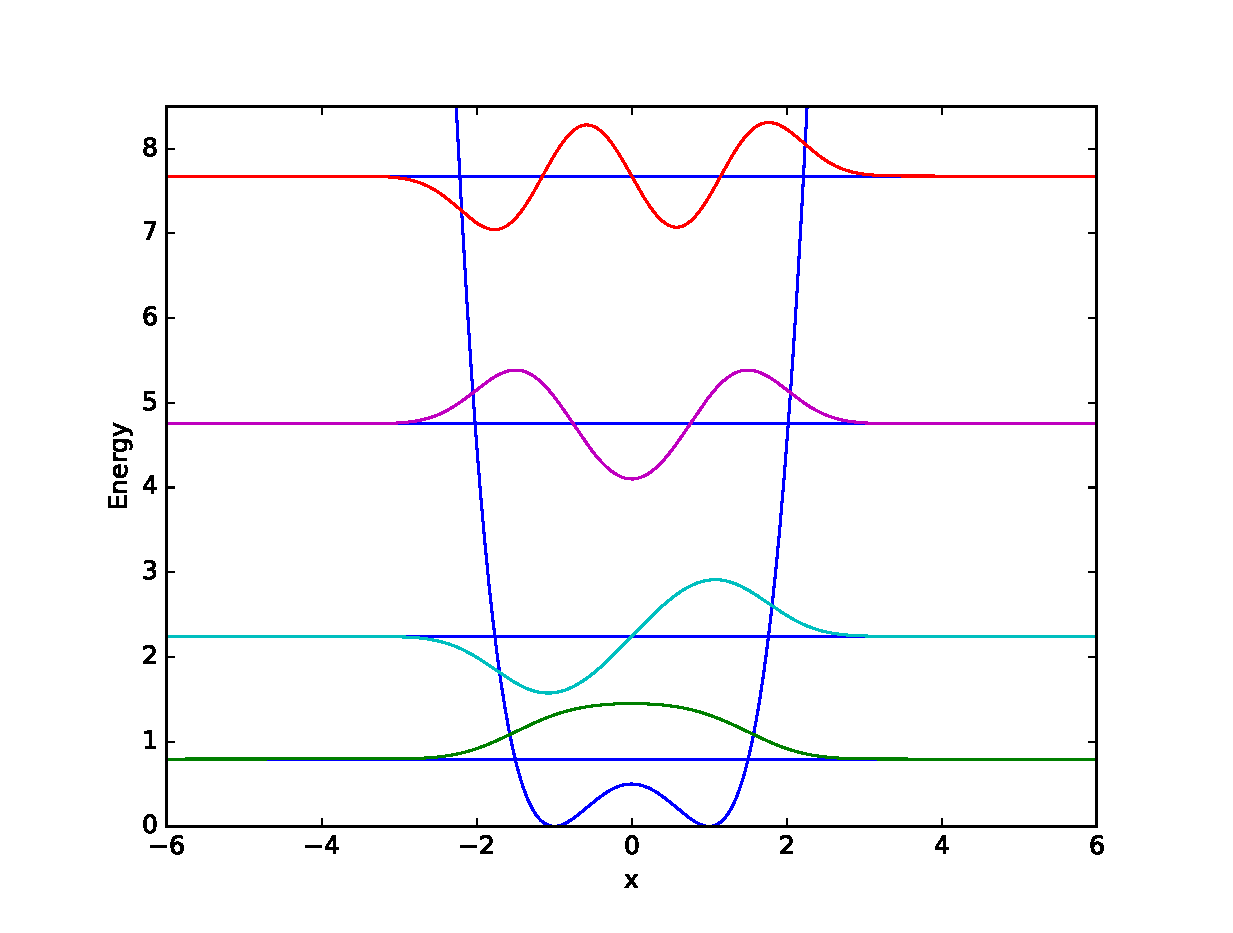
\includegraphics[width = .75\textwidth]{eigenfunctions}
\caption{Eigenfunktionen und Eigenwerte der Schrödinger-Gleichung im Doppelmuldenpotential $V(x) = 1/2(1-x^2)^2$.}
\label{fig:eigenfunction}
%
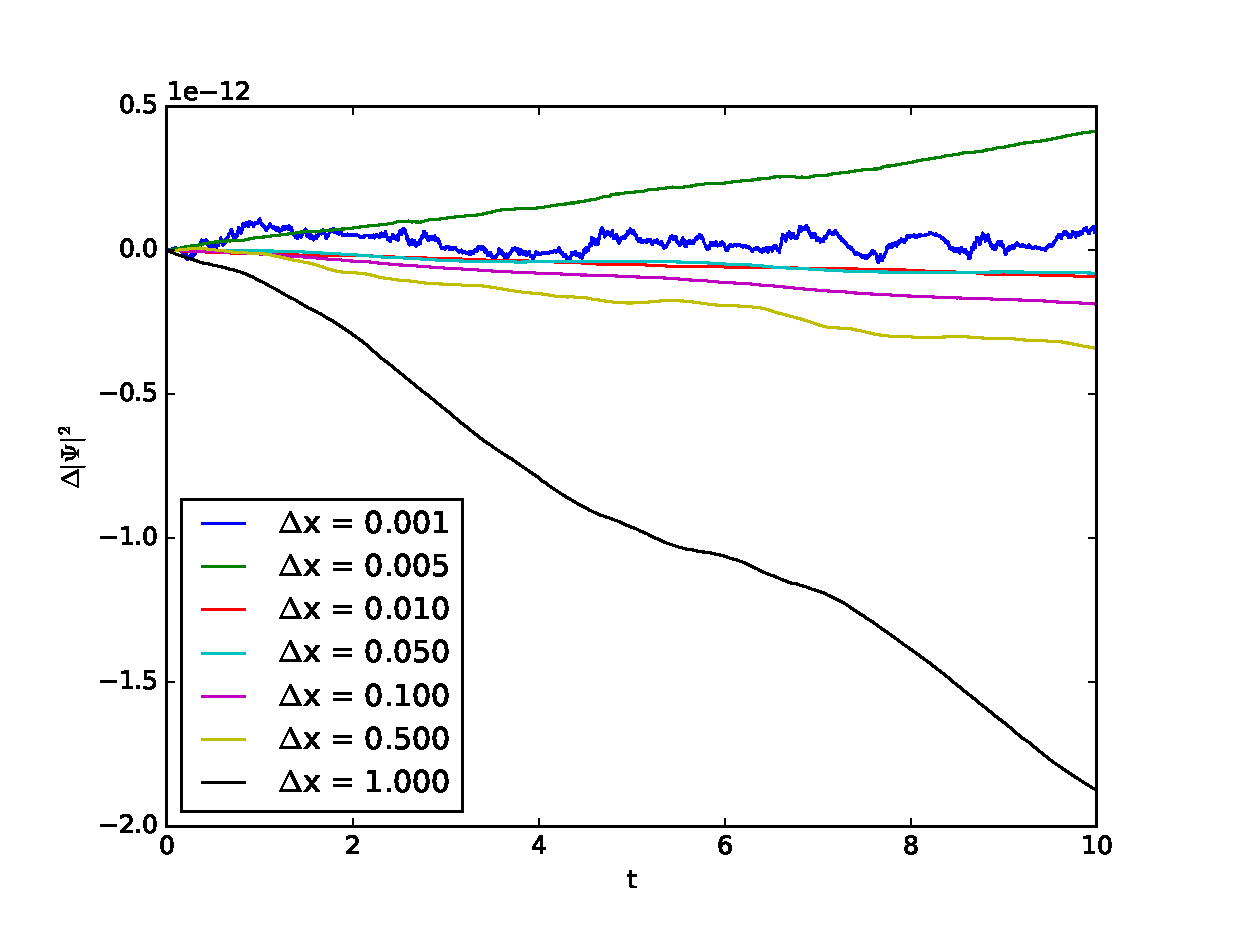
\includegraphics[width = .75\textwidth]{probability}
\caption{Änderung der Wahrscheinlichkeit $\vert \Psi \vert^2 = \int_{\mathds{R}} \vert \Psi \vert^2(x) dx$ in Abhängigkeit von der Zeit und der Schrittgröße $\Delta x$ in der Schrödingergleichung im Doppelmuldenpotential.}
\label{fig:prob}
\end{figure}
%
\begin{figure}[H]
\begin{subfigure}[b]{0.5\linewidth}
  \centering
  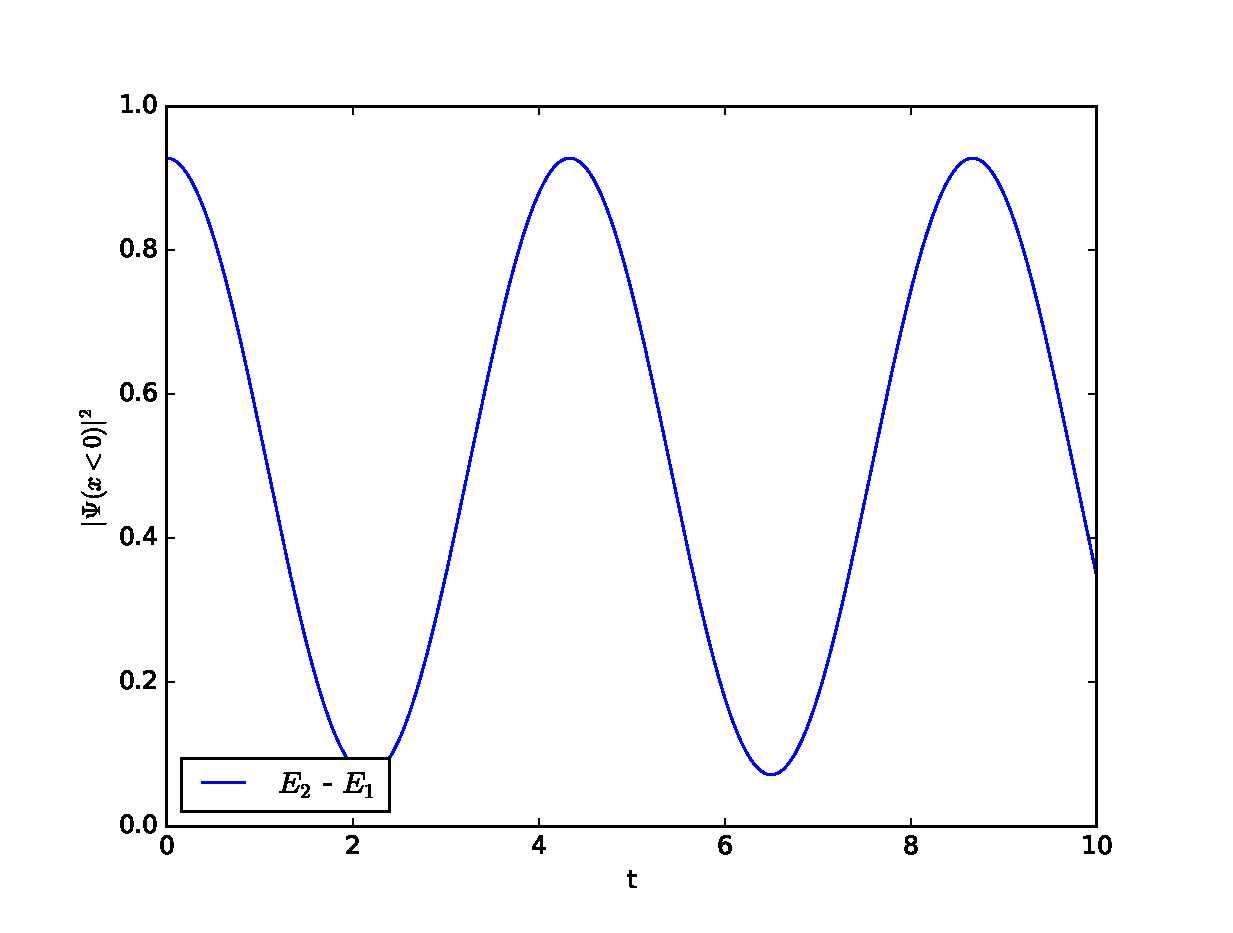
\includegraphics[width=0.9\linewidth]{probability_left21} 
  \caption{$E_2 - E_1$}
  \label{fig:21} 
  \vspace{4ex}
\end{subfigure}%% 
\begin{subfigure}[b]{0.5\linewidth}
  \centering
  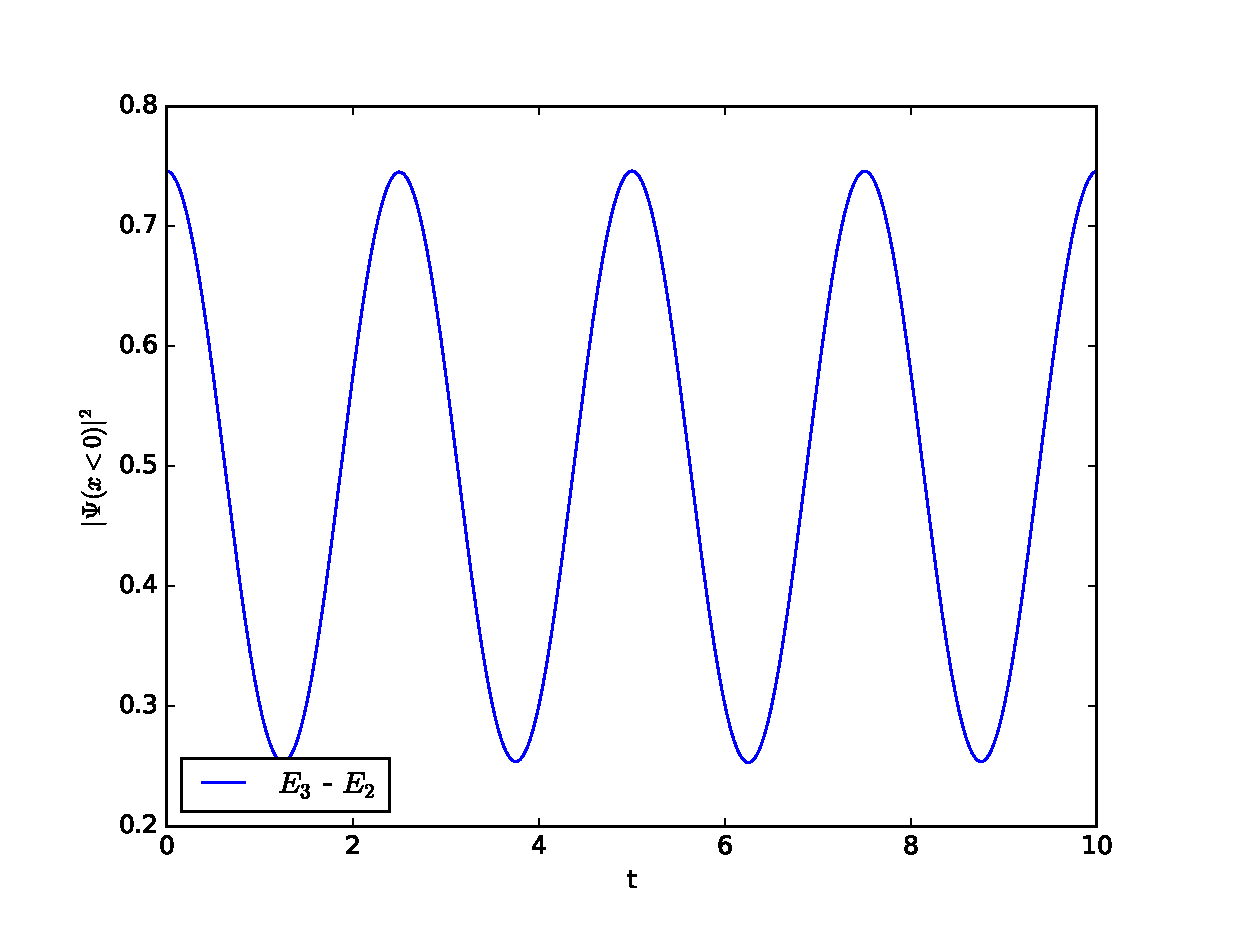
\includegraphics[width=0.9\linewidth]{probability_left32} 
  \caption{$E_3 - E_2$} 
  \label{fig:32} 
  \vspace{4ex}
\end{subfigure}
\begin{subfigure}[b]{0.5\linewidth}
  \centering
  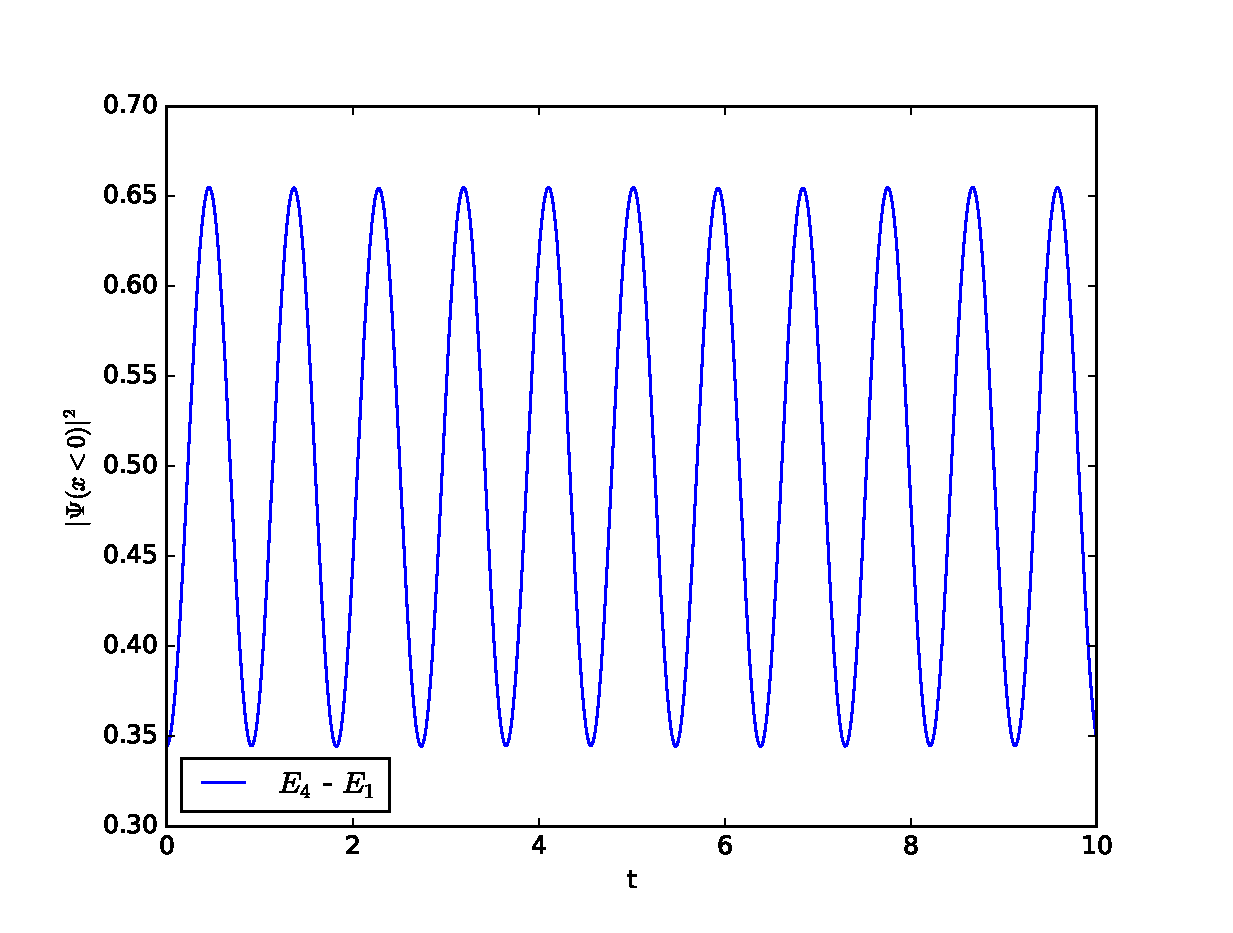
\includegraphics[width=0.9\linewidth]{probability_left41} 
  \caption{$E_4 - E_1$} 
  \label{fig:41} 
\end{subfigure}%%
\begin{subfigure}[b]{0.5\linewidth}
  \centering
  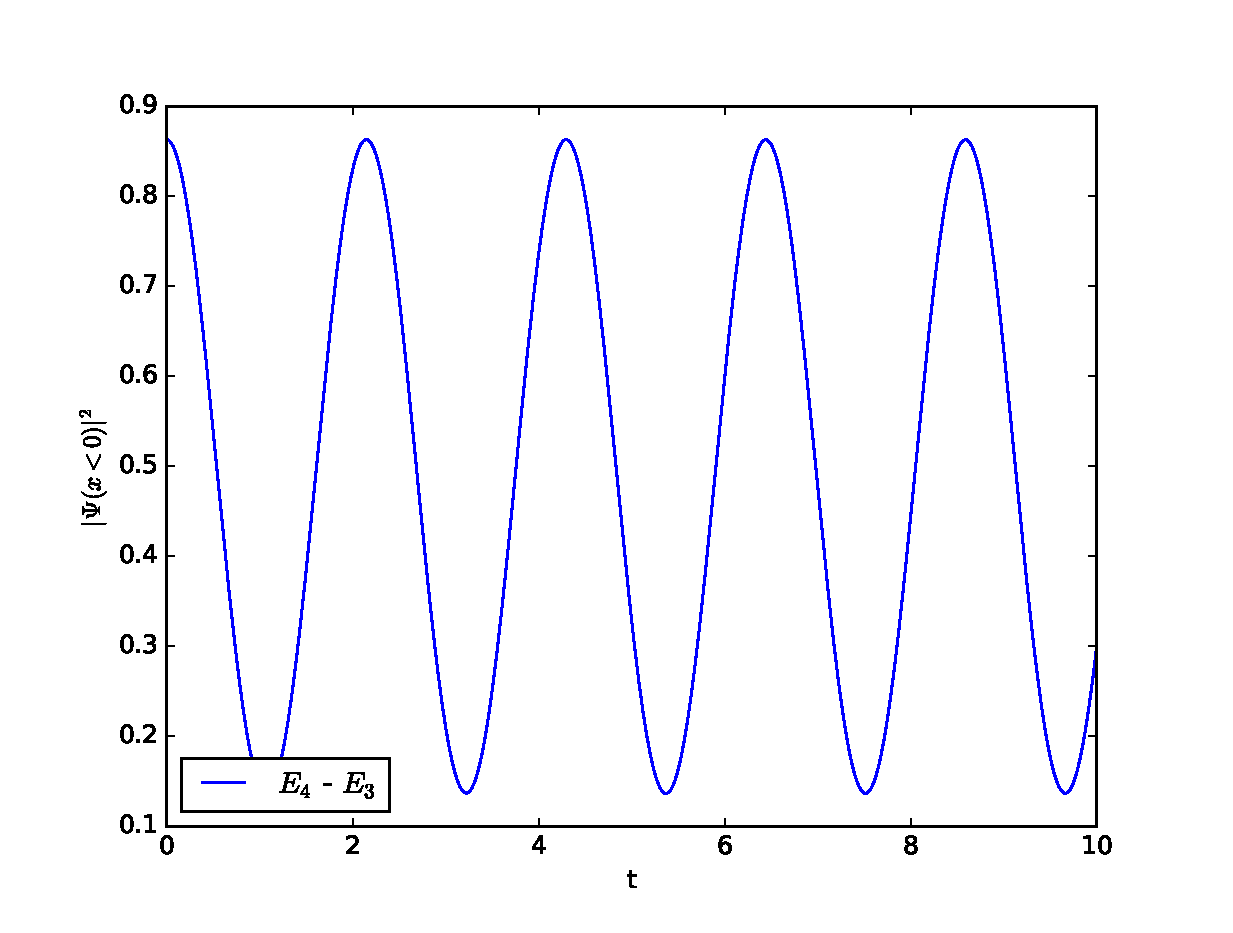
\includegraphics[width=0.9\linewidth]{probability_left43} 
  \caption{$E_4 - E_3$} 
  \label{fig:43} 
\end{subfigure}
\caption{$\vert \Psi \vert^2 (x < 0) = \int_{-\infty}^{0} \vert \Psi \vert^2(x) dx$ für Superpositionen von Eigenfunktionen der Schrödingergleichung im Doppelmuldenpotential.}
\label{fig:left_prob}
%
\centering
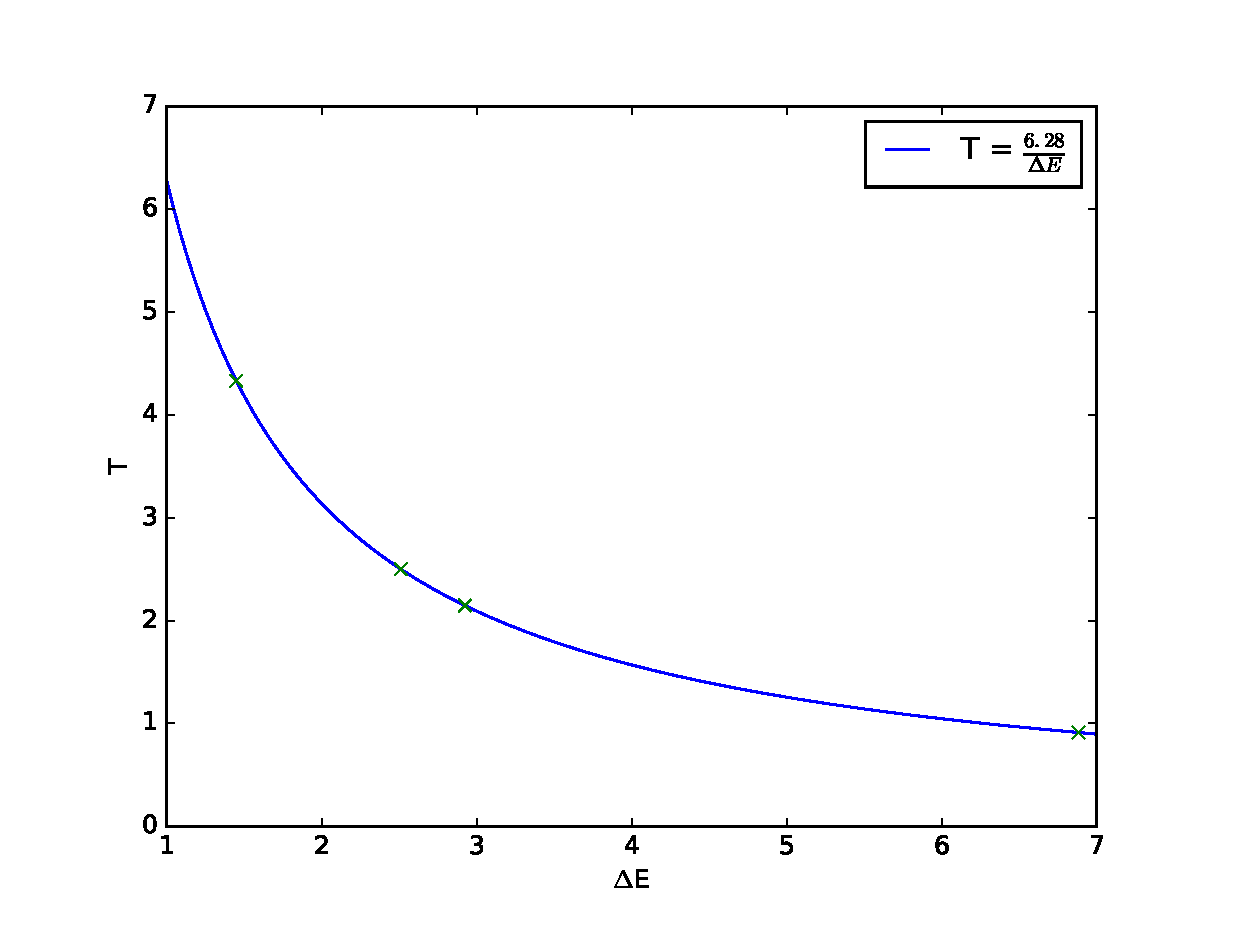
\includegraphics[width = .7\textwidth]{periodicity}
\caption{Periodizität der Wahrscheinlichkeit $\vert \Psi \vert^2 (x < 0) = \int_{-\infty}^{0} \vert \Psi \vert^2(x) dx$ in Abhängigkeit der Energie der Schrödingergleichung im Doppelmuldenpotential.}
\label{fig:period}
\end{figure}

%=======
% Code =
%=======
\newpage
\section{Code}
\subsection{Wave.py - Klasse für Schrödinger-Wellen}
\lstinputlisting[basicstyle=\footnotesize]{../code/wave.py}
\newpage
\subsection{main2.py - Programm für die Simulation und zum plotten}
\lstinputlisting[basicstyle=\footnotesize]{../code/main2.py}
\end{document}